\documentclass{article}
\usepackage[utf8]{inputenc}
\usepackage{fancyhdr}
\usepackage{lastpage}

\usepackage{float}

\usepackage{hyperref}
\usepackage{tikz} 

\usepackage[margin=3cm]{geometry}
\usepackage{amssymb}
\usepackage{amsthm}
\usepackage{amsmath}

\usepackage{pgfgantt}
\usepackage{pdfpages}


\usepackage{listings}
\lstset{
  basicstyle=\ttfamily,
  columns=fullflexible,
  frame=single,
  breaklines=true,
  postbreak=\mbox{\textcolor{red}{$\hookrightarrow$}\space},
}


\pagestyle{fancy}
\fancyhf{}


\begin{document}

\begin{titlepage}
   \begin{center}
        \large UNIVERSITY OF WARWICK\\
       \vspace*{8cm}
        \Huge UAVSI
        \\
        \vspace{0.5cm}
        \normalsize UNMANNED AERIAL VEHICLE SWARM INTELLIGENCE
        \\
        \vspace{0.2cm}
        Progress Report
            
       \vspace{5cm}

       \large \textbf{Antonio Brito}
			
			\smallskip

       \vfill

   \end{center}
\end{titlepage}

\chead{UAVSI}

\section{Background}
The uses for autonomous systems are ever-growing, with applications in logistics, agriculture, remote sensing and situational awareness\cite{muchiri}\cite{drury}. The aim of this project is to explore the use of autonomous systems in a defensive manner, specifically in the context of a swarm of Unmanned Aerial Vehicles (UAVs) in a hostile environment. The project will explore the use of swarm intelligence to ensure the survivability of the swarm in a hostile environment, where the swarm is tasked with reaching a goal location whilst avoiding obstacles and hostile entities. A model for this operation is already well defined\cite[p.183857-183858]{zhou}, where the operation of the swarm is split into several layers.

We aim to optimise the simulation of these layers, and in doing so, show the possibility for the effective operation, mission planning, obstacle avoidance and survivability of a swarm of UAVs in a challenging environment. \emph{Zhou et al.} also note the application layer of the system being malleable to the mission objective of the swarm, for applications such as in transportation and agriculture. This is an area of research that we aim to explore in the project\cite[p.183871-183872]{zhou}.

In the final report, we will also look back on findings to explore the parallels between the agents' behaviour and expected human behaviour when acting in swarms to evaluate the feasibility of future research on intelligent systems. The overall goal of the project is to combine existing technology in a novel way; in a field of research lacking open source resources.

The aim of this report is to document the progress made so far in the project, as well as outlining changes to the timetable for the project.

\section{Progress}
\label{sec:progress}
The majority of the work completed so far has been research and development of the physics model and the simulation of initial swarm behaviour, based upon Reynolds' \emph{Boids}\cite{Reynolds}.

The completed work can be split into several subsections. These sections act as the phsyical system of the simulation, as described in Fig. \ref{fig:system}. The system consists of an environment, a swarm of agents that operate within the bounds of the environment, and a positive number of agents that are part of the swarm.


\begin{figure}[H]
    \centering
    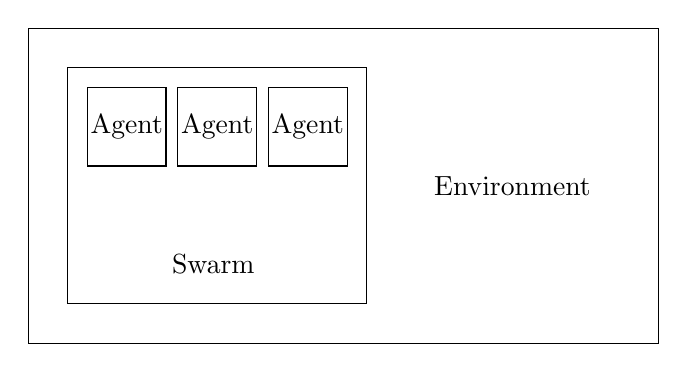
\begin{tikzpicture}
            
        \draw (0,0) rectangle (8,4);
        \draw (0.5,0.5) rectangle (4.3,3.5);
        \draw (0.75,2.25) rectangle (1.75,3.25);
        \draw (1.9,2.25) rectangle (2.9,3.25);
        \draw (3.05,2.25) rectangle (4.05,3.25);

        \node[] at (6.15,2) {Environment};
        \node[] at (2.35,1) {Swarm};
        \node[] at (1.25,2.75) {Agent};
        \node[] at (2.4,2.75) {Agent};
        \node[] at (3.55,2.75) {Agent};

    \end{tikzpicture}
    \caption{System Diagram}
    \label{fig:system}
\end{figure}

\subsection{Agent}
A model simulating the movement and physics of a quadcopter operating in an Earth-like environment has been developed. This has been achieved by simulating a quadcopter as a rigid body, with four \emph{`propellers`}\footnote{For the purposes of the simulation, the propellers do not rotate. Thrust is simulated as an upward force.} generating thrust. At this stage, some constants have been assigned to the model in order to simulate operation in an Earth-like environment. These constants may be refined as the project progresses if needed. The table of these constants is seen in the table below.

To gain familiarisation with the \emph{Unity Engine}, the initial aim was to operate the quadcopter using keyboard controls, rather than autonomously. The design of the control system and model was largely based on \emph{Luukkonen's} research in the field\cite{Luukkonen} alongside some high-level explanatory reading in \emph{IJREAM}\footnote{International Journal for Research in Engineering Application \& Management}\cite{Tatale}.

The keyboard operation was based on 8 axes of control. These are summarised in Table \ref{tab:keyboard-operation}.

\begin{table}[H]
    \centering
    \begin{tabular}{|c|c|}
        \hline
        \textbf{Operation} & \textbf{Key} \\
        \hline
        Positive Pitch & W \\
        \hline
        Negative Pitch & S \\
        \hline
        Roll Left & A \\
        \hline
        Roll Right & D \\
        \hline
        Yaw Clockwise & L \\
        \hline
        Yaw Anticlockwise & J \\
        \hline
        Ascend & I \\
        \hline
        Descend & K \\
        \hline
    \end{tabular}
    \caption{Keyboard Drone Operation}
    \label{tab:keyboard-operation}
\end{table}

This then allowed for a control system to be tested. The aim of this system was to allow for the drone to be controlled in a stable manner, with the drone returning to a stable position when no controls were being applied. This was achieved by using a \emph{PID} controller\cite[p.72-73]{Szafranski}. Whilst there was some success from the literature, the implementation of the controller largely came from online tutorials, namely from \emph{Carbon Aeronautics}\cite{Carbon}.

A \emph{PID} controller is a control loop feedback mechanism, with three main constants. \emph{P}, the proportional constant, produces an output that is directly proportional to the error at the current time. However, this alone may result in an unstable system where the agent overshoots the target position. Hence, the \emph{I} and \emph{D} constants are used to counteract this.

\emph{I}, the integral constant, considers the sum of the errors over time. This reduces the amount of \emph{steady-state error}, defined as the distance between the input and output response as time tends to infinity.

\emph{D}, the derivative constant, considers the rate of change of the error, with the aim of reducing overshoot error. The output of the controller is then the sum of the three constants multiplied by their respective error values. The \emph{PID} controller underwent empirical tuning whereby the initial adjustment involved setting the \emph{P} constant to an elevated value, progressively attenuating it until achieving stability in the drone's behavior. Subsequently, the iterative refinement of the \emph{I} and \emph{D} constants followed a similar approach to achieve optimal controller performance. This was achieved by observing the drone's behaviour in the \emph{Unity} editor, as well as the console output of the controller's error values. It should be noted that this isn't the optimal tuning method, and mathematical methods exist to tune the constants\cite[p.67]{evans}. This may be a later consdieration if the control system becomes unstable. However, at this time, the system is stable.

The provisional final values of the constants are shown in Table \ref{tab:pid-constants}.

\begin{table}[H]
    \centering
    \begin{tabular}{| c | c | c | c |} 
    \hline
    Control Operation & $K_p$ & $K_i$ & $K_d$ \\ 
    \hline
    Thrust & 6 & 5 & 2 \\
    \hline
    Pitch & 10 & 10 & 2 \\
    \hline
    Roll & 10 & 10 & 2 \\
    \hline
    Yaw & 10 & 10 & 2 \\
    \hline
    \end{tabular}
    \caption{Tuning Constants}
    \label{tab:pid-constants}
\end{table}


\subsection{Swarm}

The initial work surrounding the operation of the swarm has been completed. This consists of the three separate \emph{Boids} behvaiours - alignment, cohesion and separation\cite{Reynolds}. Combining these three behvaiours and tuning their respective influences for effective swarm operation has not yet been completed. This has been reflected in the outline of the revised project timetable.

Additionally, the mathematical model of the swarm's operation itself has not been completed. Currently, high-level methods are being used to control the individual behaviours, namely \emph{Unity's} \verb|transform.worldToLocalMatrix| method. This is used to create a transformation matrix in the local coordinate frame of the agent, which is then used to calculate the desired direction of movement. This is not ideal, as it is not a true mathematical model of the swarm's operation. Ideally, this will be expanded to utilise quarternions to model the rotation of an agent. So far, \emph{3Blue1Brown}'s interactive guide has proven useful in understanding the mathematics behind quarternions\cite{3Blue1Brown}. The complexity in understanding quarternions has been reflected in the revised timetable.

\subsection{Environment}
The initial project noted the development of the environment would be partly done in parallel with the physics model and completed before the work on pathfinding. With some discussions, it was decided that as the environment may partly constitute an obstacle, the major work on creating a complex and noisy environment would be completed after the work on pathfinding, at the stage of working on collision avoidance. This is reflected in the revised timetable.

In place of this, an initial environment was completed, formed of a simple ground plane. There are currently plans to create a randomly assigned goal location within the dimensions of the plane to allow for the development and testing of the pathfinding algorithms.

\section{Project Management}
\label{sec:timetable}

Generally, the management of the project so far has been successful. As with any project, there have been delays, which have been mitigated by effective risk planning and management. The delays are explained alongside the revised timetable. In spite of this, the project's development is consistent, largely in part due to being held to account by regular, usually weekly, meetings with the project supervisor.

At this stage, it is useful to outline the timetable changes. These are seen in Figure \ref{fig:gantt}.

\begin{figure}[H]
    \begin{center}
    \begin{ganttchart}[y unit title=0.5cm,
    y unit chart=0.6cm,
    vgrid,hgrid, 
    title label anchor/.style={below=-1.6ex},
    title left shift=.05,
    title right shift=-.05,
    title height=1,
    progress label text={},
    bar height=0.7,
    group right shift=0,
    group top shift=.6,
    group height=.3,
    group peaks height=.2,
    link mid=.45,
    progress=today,
    today=8]{1}{24}
    %labels
    \gantttitle{Term 1}{10}
    \gantttitle{Xmas Break}{4}
    \gantttitle{Term 2}{10} \\
    \gantttitle{1}{1} 
    \gantttitle{2}{1} 
    \gantttitle{3}{1} 
    \gantttitle{4}{1} 
    \gantttitle{5}{1}
    \gantttitle{6}{1} 
    \gantttitle{7}{1} 
    \gantttitle{8}{1} 
    \gantttitle{9}{1} 
    \gantttitle{10}{1}
    \gantttitle{1}{1} %week 11
    \gantttitle{2}{1} 
    \gantttitle{3}{1} 
    \gantttitle{4}{1} 
    \gantttitle{1}{1} %week 15
    \gantttitle{2}{1} 
    \gantttitle{3}{1} 
    \gantttitle{4}{1} 
    \gantttitle{5}{1}
    \gantttitle{6}{1} %week 20
    \gantttitle{7}{1} 
    \gantttitle{8}{1} 
    \gantttitle{9}{1} 
    \gantttitle{10}{1} \\
    %tasks
    \ganttgroup{Supplementary Work}{1}{24} \\
    \ganttbar{Project Spec}{1}{2} \\
    \ganttbar{Progress Report}{8}{8} \\
    \ganttbar{Presentation}{22}{24} \\
    \ganttbar{Informing Future Work}{22}{24} \\

    \ganttgroup{Swarm Operation}{2}{9} \\
    \ganttbar{Physics Model Research}{2}{3} \\
    \ganttbar{Simple Environment}{2}{3} \\
    \ganttbar{Physics Model Development}{3}{6} \\
    \ganttbar{Swarm Behaviour}{6}{9} \\
    \ganttbar{Evaluation}{8}{9} \\

    \ganttgroup{Pathfinding}{11}{16} \\
    \ganttbar{A* \& D* in 2D}{11}{12} \\
    \ganttbar{3D Implementation of D*}{13}{14} \\
    \ganttbar{Swarm Leader Navigation}{12}{14} \\
    \ganttbar{Leaderless Navigation}{13}{15} \\
    \ganttbar{Complex Environment}{15}{16} \\
    \ganttbar{Evaluation}{15}{16} \\

    \ganttgroup{Project Extensions}{17}{24} \\
    \ganttbar{Obstacle Avoidance}{17}{19} \\
    \ganttbar{Obstacle Detection}{19}{21} \\
    \ganttbar{Hostile Obstacles}{22}{23} \\
    \ganttbar{Winged Aircraft}{24}{24}

    \ganttlink{elem8}{elem12}
    \ganttlink{elem12}{elem13}
    \ganttlink{elem12}{elem14}
    \ganttlink{elem17}{elem3}
    \ganttlink{elem10}{elem3}


    \end{ganttchart}
    \end{center}
    \caption{Revised Gantt Chart. Numbers shown are week numbers.}
    \label{fig:gantt}
\end{figure}

The changes to the timetable can be grouped and summarised as the following:

\subsection{Swarm \& Agent Physics}
As explained in Section \ref{sec:progress}, the development of the swarm model has proven more complex than expected. As such, the expected timeframe for completion of this group of tasks (Swarm Operation) has been extended by 3 weeks. This is to allow for the completion of the swarm model, as well as the evaluation of the swarm's operation, which has mostly been completed in parallel, partly owing to the delays in the swarm model's development.

Secondly, a new task has been added to the chart - \emph{Swarm Behaviour}. This is a subset of the \emph{Physics Model} task, with a greater focus on getting the swarm to act in a stable manner.

\subsection{Change to Environment Development}
The decision to split the stage of development focusing on the environment model into two distict stages, namely \emph{Simple Environment} and \emph{Complex Environment} in Fig. \ref{fig:gantt} has warranted the need for a new task in the chart to achieve the latter half of the split. This has meant a slight shift in the \emph{Pathfinding} task group.

\subsection{Project Extensions}
Lastly, the timeframes for the tasks within the project extension task group have been shortened. This is to allow for more time spent on earlier, more vital tasks. This was accounted for in the risk assessment, as part of the project specification.

\section{Ethics}
As noted previously in the project specification, there are no ethical concerns with the project. The project is purely a simulation, and as such, there are no concerns with human involvement or the usage of personal data. However, at this stage, it should be noted that the project deals with artificial intelligence, namely autonomous systems. Notably, the Students' Union passed a motion in 2023 which aimed to lobby the University to \emph{`form an internal Research Ethics Committee for Computer Science and AI, in order to assess and mitigate the risk that university dual-use research could be applied for unintended malicious uses or incorporated in harmful weapons systems, such as autonomous weapons systems'}\cite{WSU}. This is a reccomendation that should be considered by the department.

\section{Conclusion}

Generally, we note that the project is on track. The main changes in the timetable reflect minor delays and changes in the order of tasks. As such, the project is still expected to finish on time.

\newpage

\bibliographystyle{IEEEtran}
\bibliography{refs}

\LARGE
\bigskip
\centering
\textbf{Appendix: Project Specification Overleaf}

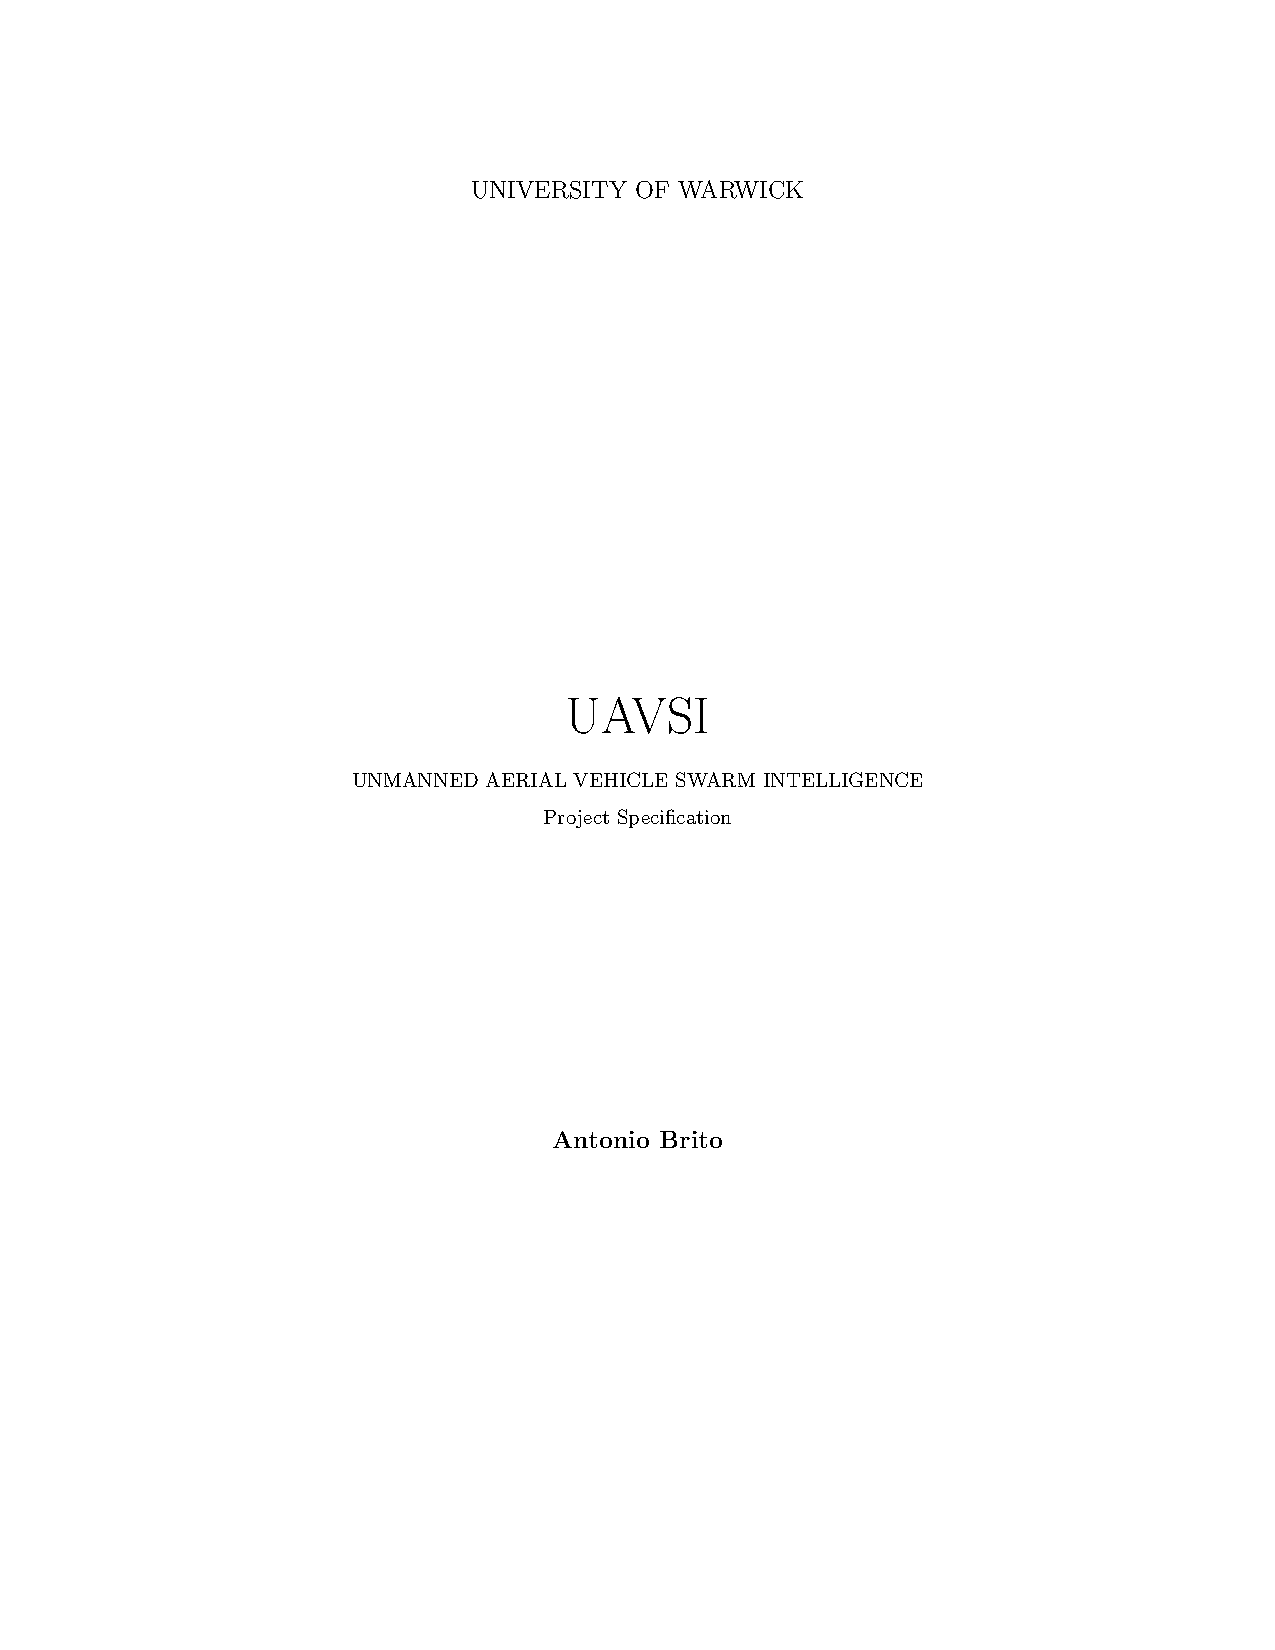
\includepdf[pages=-]{../project-specification/pspec.pdf}

\end{document}